%************************************************
\section{Black-box Analysis}\label{ch:Blackbox}
%************************************************
When developing a software system, it often happens that we need different frameworks or other systems to develop ours.
While it would be possible to develop these systems ourselves, in most cases this is inefficient and slows down the release of our system.
To speed up this process, we can use other systems that are already available to us, this however introduces us to the issue whether the system 
also fulfills our needs besides functionality, for example performance. 

For this purpose, we can perform a black-box analysis of the system. 
A black-box analysis is conceptually simple, given a configurable system, we select a configuration that contains the feature we are interested in. 
We run the system with different configuration containing the features we are interested in,
during execution we measure the non-functional properties we can observe.
Next, we use these measurements to build a performance-influcence model, that becomes more accurate as the number of unique configurations measured increases. 
Since it is not feasible to measure all possible configuration, we use our model to predict the time it takes to run a configuration
having to run the configuration on the system.


\begin{figure}[h]
    \centering
    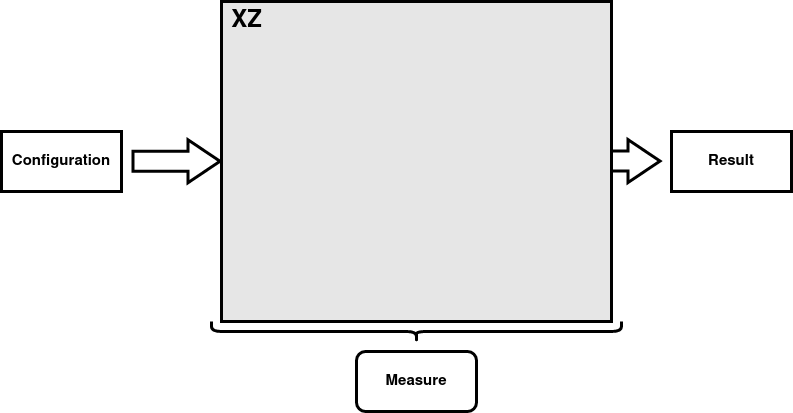
\includegraphics[scale=0.6]{gfx/BlackBoxXZ.png}
    \caption{A Black-box Version of xz}
    \label{fig:BBxz}
\end{figure}

As an example for a black-box analysis we modify xz from \ref{fig:xz}. To perform a black-box analysis we feed xz with the different configuration that
contain the features we choose to measure. Now, for each configuration we observe the properties we are interested in, such as time spend during the 
execution of the system, how xz produces these result we cannot tell. After repeating this process multiple time we use all the measurements collected to 
build a performance-influcence model that represents xz.


\subsection{Collecting data}

Let us now proceed on how we collect data. First, we analyze the configuration space using our feature model introduced in Chapter \ref{ch:Feature Model}
and decide on the set of features we want to analyze. To deal with the effects of combinatorial explosion, we select a subset of the entire
configuration space and analyze it using a brute force approach, rather using sampling strategies which would exceed the scope of this
thesis.

In addition, we will only use valid configurations that satisfy the constraints of our feature model, to mitigate
the influence that colinear features have or our model.

\subsection{Disadvantages of black-box model}
Even though a black-box analysis is simple in nature, it faces two major challenges, namely combinatorial explosion and collinear features, both need to be
handled carefully in order to build an accurate performance-influence model.

\paragraph{Combinatorial Explosion}
One of the larger problems we face when using black-box models is the issue of combinatorial explosion, 
which refers to the effect that when features increase linearly, the number of possible configuration and thus system variants,
increase exponentially \cite{Combinatorial-explosion}.

Suppose we have a configurable system where each feature is a binary option that you can either select or deselect. We also define 
that in this system each feature is completely independent of another, (i.e. the system has no constraints and selecting or deselecting a featureMuss
has no effect on other features). The number of unique configurations this system can produce is $2^n$, where $2$ refers to
the type of feature options allowed, binary in our case and $n$ denotes the number of features. 

Here lies the problem, all these different features might interact with each other in different ways, and for very small systems,
we can certainly brute-force our way by benchmarking all possible configuration, however this does not scale, it is already not feasible for 
larger systems. As an example, the Linux kernel contains 10000 different features \cite{Linux-Kernel}, for reference it is estimated that the universe
contains about $10^79$ atoms, which is still less than the variants of a system with 263 features, it is already impossible to use brute-force to analyze
such as system, let alone the Linux kernel.

For this reason, we cannot fully explore the entire configuration space 
and therefore need to select a subset that represent the system with a high accuracy. To do that state of the art black-box model use sampling
strategies to find a suitable subset, such as, pair-wise sampling, most-enabled-disabled and random sampling.

\paragraph{Multicollinear Features}\label{ColinearF}
We have already mentioned that features that do not influence each other are called independent features, but configurable systems are composed
of not only independent features. If there is a dependence between more than two features, we call these features multicollinear.

The reason why multicollinearity is a problem in a black-box analysis is
that we can only observe nun-functional properties during execution and are unable to correctly assign the influence of each feature
on the system. One way multicollinearity is introduced into a system is by using alternative groups, since the selection of a feature in the
alternative group depends on which options are chosen by the other features in that group. \cite{Multicollinearity}
\pagebreak

\begin{table}[h]
    \centering
    \begin{tabular}{llllll}
    \hline
    Base & A & B & C &  & $\bm{\Pi(*)}$ \\ \hline
    1 & 1 & 0 & 0 &  & $\mathbf{5}$  \\
    1 & 0 & 1 & 0 &  & $\mathbf{10}$  \\  
    1 & 0 & 0 & 1 &  & $\mathbf{15}$  \\\hline
    \end{tabular}  
    \caption{Configuration example illustrating multicollinearity in an alternative group}\label{tab:alternative}
\end{table}

Now consider the example of \ref{tab:alternative}, where we see a configuration example that contains multicollinear features due to an alternative group.
The example contains a Base feature and 3 features for an alternative A, B, and C, which means only one these 3 features can be selected for each
configuration.
This now clearly shows the dependency between these features, because for feature C to be selected, B and C needs to be deselected, which means
$C = 1 - B - C$ needs to be satisfied. 

\begin{align*}
    \Pi(c) &= 0 + 5 \cdot c(A) + 10\cdot c(B) + 20\cdot c(C) \\
    \Pi(c) &= 5 + 10 \cdot c(A) + 5\cdot c(B) + 20\cdot c(C) \\
    \Pi(c) &= 8 + 20 \cdot c(A) + 10\cdot c(B) + 7\cdot c(C) \\
\end{align*}

This, leads us to multiple performance-influcence model that are accurate regarding each measurement, but when we
compare them state completely different things. 
The problem here is that since one child of the alternative must be selected, but the other are deselected, we cannot correctly infer the influence
all features has on to the system as we can see in our example base is attributed $0$, $5$ and $8$. 
These values of base or the selected feature can be set in any ratio, as long as the sum of the two is equal to the time we measured.

A different way multicollinearity is introduced into the system is when we have features that are mandatory or connected by a condition. 
If we have features that are mandatory, we are unable to distinguish these features with our black-box analysis because they are always selected
together, we are unable to determine the extent to which each feature influences the system. \cite{Multicollinearity}

\begin{algorithm}[h]
    \caption{Equivalence \label{alg:Colinear}}
    \begin{algorithmic}[1]

    \If{$(c \textit{ and }  \lnot d) or (\lnot c \textit{ and } d)$} 
        \State $c,d \gets False$
    \EndIf

    \end{algorithmic}
    \end{algorithm}

Extending the example code from \ref{alg:performanceExample} with an additional condition where $C \equiv D$ holds, so that 
either C or D can be selected without the other, we insert the code snippet \ref{alg:Colinear} after \ref{alg:code_insertion}.

Now, if we select a configuration c containing the features \{\{A\}, \{B\}, \{C\}\} we get multiple {\perfInfluenceModel}s:

\begin{align*}
    \Pi_1(c) &= 1 + 1\cdot c(C) + 1 \cdot c(D) + 1\cdot c(C) \cdot c(D) \\
    \Pi_2(c) &= 1 + 0\cdot c(C) + 0 \cdot c(D) + 3\cdot c(C) \cdot c(D) \\
    \Pi_3(c) &= 1 + 1\cdot c(C) + 2 \cdot c(D) + 0\cdot c(C) \cdot c(D) \\
\end{align*}

All the {\perfInfluenceModel}s are accurate with respect to the measurements, but assign different values to each feature. 
In $\Pi_1(c)$ and $\Pi_2(c)$, all features are assigned different values from what we would expect when looking at \ref{alg:performanceExample},
while the \perfInfluenceModel of $\Pi_C(c)$ assigns the expected values.

\subsection{Creating a Performance-Influence Model using Multiple Linear Regression}
We use our black-box model by feeding it inputs and meassuring the time it takes the system to produce a output. From this 
very limited set of data, we now need to bulid our performance-influence model, which we do by using multiple linear regression.
We use multiple linear regression beacause the formular we learn can be understood by us humans, unlike other approaches like neural networks.
Moreover, to use multiple linear regression, we do not need to know anything about the inner workings of the system,
which benefits our black-box model. \cite{Linear-Regression-Performance}

We use the following formular of linear regression for matrices\cite{Linear-Regression-Performance}:

\begin{align*}
        y &= \beta_0 + \beta_1 x_1 + \beta_2 x_2 ... \beta_n x_n + \epsilon   \\
        y &= X \beta + \epsilon
\end{align*}


Where $y$ is called dependendent variable and $X$ is called independent variable $y$ in our case is a vector with n elements containing
the output of our black-box model, i.e. the time meassurement generated for each feature configuration in our feature set. What we
are intrested in are the values of the coefficents $\beta$, since they quantify the influence of each feature or feature interaction
on to the whole system. In addition, $\beta_0$ denotes the intercept, which for us represents the influence of the base code, meaning
the part of the code that gets exectued regardless of the selected feature configuration.
Our independent variable $X$ is a $n \times m$ martrix, where $n$ is the number of configurations used and $m$ the powerset of all
features. The reason we use a powerset here is to model all feature interactions in our matrix.
The value of each feature in the matrix is either $1$ if the feature is selected, or $0$ if its not. If we have numerical features with $l$
different options, we split this features into $l$ binary features and encode them as an alternative group in our feature model.
For all our meassurements we also have a possible error represented by $\epsilon$. \cite{Linear-Regression}

%To Do superset features

